\secrel{Финальная схема датчика темноты}

Функция \term{входной} части схемы\ --- определение уровня освещенности.

Функция \term{преобразующей} части схемы (транзистор)\ --- усиление
небольшого изменение напряжения из-за легких изменений освещенности.

Функция \term{выходной} части цепи\ --- индикация для пользователя.

Функция \term{источника питания}\ --- надежно обеспечить энергию для работы
схемы.

\bigskip 
Когда темно, светодиод включается, когда свет присутствует, светодиод выключен.
Эта схема может использоваться как игрушка для ребенка, чтобы ориентироваться в
темноте, и найти дверь в темной комнате.

\emph{Диод}, \emph{светодиод} и \emph{транзистор} поляризованные элементы, т.е.
имеют положительные и отрицательные выводы и, следовательно, требуют правильного
включения в схему, или они не будут работать.

\bigskip
Вы можете определить полярность светодиода найдя спил на корпусе (отрицательный
вывод, катод) или по длинной ноге (положительный вывод, или анод)

Полярность \emph{транзистора} можно определить за счет формы корпуса и зная
расположение трех выводов.

\bigskip Нарисуйте линии от компонентов к их символам на схеме, чтобы помочь вам
запомнить их. Помните, что резистор в выходной цепи был установлен с более
низким значением (уменьшен от 1k до 390\,Ом) чтобы в окончательной схеме сделать
светодиод ярче.

\bigskip\noindent
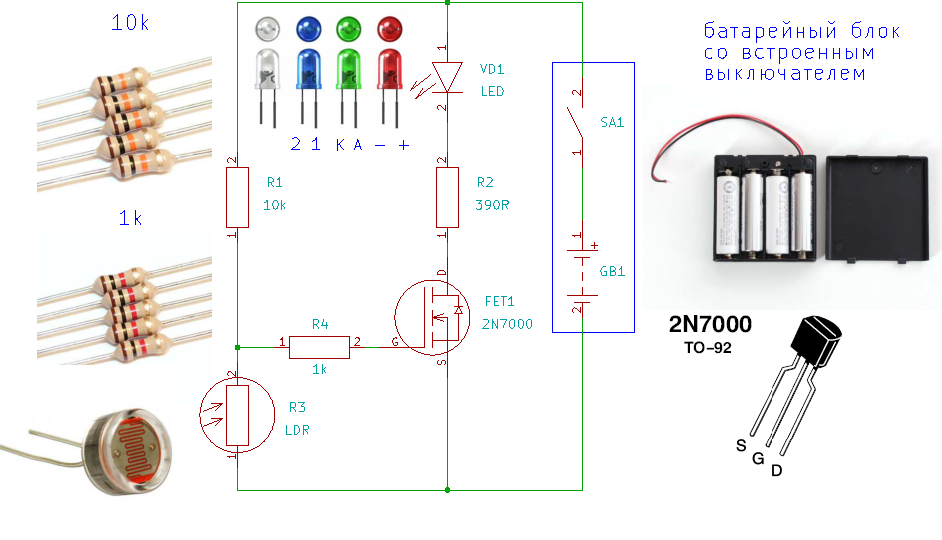
\includegraphics[width=\textwidth]{bcollis/ldr/final.pdf}
